% Report adapted from the UFAM template supplied by the group.
\documentclass[a4paper,12pt,espacoumemeio,normaltoc,noheader,openany]{abntengmecufam}
% Packages and layout for the technical report; the original class is preserved.
\usepackage[T1]{fontenc}
\usepackage[utf8]{inputenc}
\IfFileExists{brazilian.ldf}
  {\usepackage[brazilian]{babel}}
  {\usepackage{babel}\babelprovide[main,import=pt-BR]{brazilian}}
\usepackage{amsmath}
\usepackage{txfonts}
\usepackage{microtype}
\usepackage[left=3cm,right=2cm,top=3cm,bottom=2cm]{geometry}
\usepackage{graphicx}
\usepackage{xcolor}
\usepackage{booktabs,longtable,tabularx,array}
\usepackage{ragged2e}
\usepackage{enumitem}
\usepackage{float}
\usepackage{placeins}
\usepackage{listings}
\usepackage{tikz}
\usetikzlibrary{arrows.meta,positioning,calc,fit,backgrounds,shapes.geometric}
\usepackage[font=small,labelfont=bf,labelsep=endash]{caption}
\usepackage{url}
\usepackage[unicode,hidelinks]{hyperref}
\usepackage[alf]{abntex2cite}

% Use the actual hyperlink targets instead of the legacy class's TOC targets.
\renewcommand{\ABNTaddcontentsline}[3]{%
  \ifthenelse{\boolean{ABNTNextOutOfTOC}}
    {\setboolean{ABNTNextOutOfTOC}{false}}
    {\addcontentsline{#1}{#2}{#3}}}

\renewcommand{\thesection}{\arabic{section}}
\renewcommand{\thesubsection}{\thesection.\arabic{subsection}}
\renewcommand{\theequation}{\arabic{equation}}
\setcounter{secnumdepth}{2}
\setcounter{tocdepth}{2}
\setlength{\parindent}{1.25cm}
\setlength{\parskip}{0.12cm}
\setlength{\emergencystretch}{1.5em}
\setlength{\tabcolsep}{5pt}
\renewcommand{\arraystretch}{1.15}
\setlist[itemize]{leftmargin=1.2cm,itemsep=2pt,topsep=4pt}
\setlist[enumerate]{leftmargin=1.2cm,itemsep=2pt,topsep=4pt}
\newcolumntype{L}[1]{>{\RaggedRight\arraybackslash}p{#1}}
\newcolumntype{Y}{>{\RaggedRight\arraybackslash}X}
\newcommand{\source}[1]{\par\smallskip{\footnotesize\noindent Fonte: #1.\par}}
\newcommand{\celsius}{\ensuremath{\,^{\circ}\mathrm{C}}}
\newcommand{\modelversion}{\texttt{embedded-rf-6b0d1696547d}}
\lstset{basicstyle=\ttfamily\footnotesize,columns=fullflexible,
  breaklines=true,breakatwhitespace=false,showstringspaces=false,
  frame=single,rulecolor=\color{black!30},numbers=left,numberstyle=\tiny,
  numbersep=7pt,xleftmargin=0.5cm,framexleftmargin=0.3cm,
  captionpos=t,aboveskip=10pt,belowskip=10pt}
\renewcommand{\lstlistingname}{Código}
\tikzset{
  block/.style={draw=black!70,rounded corners=2pt,fill=blue!3,
    align=center,font=\small,minimum height=1.1cm,inner sep=6pt},
  decision/.style={diamond,aspect=2.7,draw=black!70,fill=orange!6,
    align=center,font=\small,inner sep=2pt},
  flow/.style={-{Latex[length=2.2mm]},line width=0.65pt},
  terminal/.style={block,rounded corners=8pt,fill=black!4,minimum height=0.65cm},
  edge label/.style={font=\footnotesize,fill=white,inner sep=2pt}
}


\newcommand{\ReportTitle}{MS-Monitor: arquitetura de monitoramento e classificação embarcada de condições de armazenamento de grãos}
\newcommand{\ReportAuthors}{Camila Amorim dos Santos\\Gabriel dos Santos Tavares\\Gabriel Iuji Oliveira Taguchi\\Jéssica Corsino Ribeiro\\Nathália Garcez Galindo Brandão}
\newcommand{\ReportTeacher}{Prof. Dr. Carlos Alberto Oliveira de Freitas}
\newcommand{\ReportPlace}{Itacoatiara--AM}
\newcommand{\ReportYear}{2026}

\hypersetup{pdftitle={MS-Monitor: arquitetura de monitoramento e classificação embarcada},
pdfauthor={Grupo 03 - Inteligência Artificial Embarcada},
pdfsubject={Segundo trabalho: relatório técnico do protótipo MS-Monitor}}

\begin{document}
\hypersetup{pageanchor=false}
\begin{titlepage}
\thispagestyle{empty}
\begin{center}
\begin{minipage}[c]{0.13\textwidth}

\includegraphics[width=\linewidth]{Imagens/brasaocor2.jpg}
\end{minipage}\hfill
\begin{minipage}[c]{0.69\textwidth}
\centering\small
UNIVERSIDADE FEDERAL DO AMAZONAS\\
INSTITUTO DE CIÊNCIAS EXATAS E TECNOLOGIA\\
PROGRAMA DE PÓS-GRADUAÇÃO EM\\
CIÊNCIAS, TECNOLOGIA E SAÚDE
\end{minipage}\hfill
\begin{minipage}[c]{0.13\textwidth}

\includegraphics[width=\linewidth]{Imagens/brasao_PPGCTS.png}
\end{minipage}
\vspace{1.0cm}

{\large Inteligência Artificial Embarcada}\\
Segundo trabalho --- Grupo 03

\vspace{1.4cm}
{\normalsize\ReportAuthors\par}

\vfill
{\Large\bfseries\ReportTitle\par}
\vfill

{\ReportPlace\\\ReportYear\par}
\end{center}
\end{titlepage}

\begin{titlepage}
\thispagestyle{empty}
\begin{center}
\ReportAuthors

\vspace{2cm}
{\Large\bfseries\ReportTitle\par}
\end{center}
\vspace{1.7cm}
\begin{flushright}
\begin{minipage}{0.62\textwidth}
\setstretch{1.0}
Relatório técnico apresentado como segundo trabalho da disciplina Inteligência
Artificial Embarcada, do Programa de Pós-Graduação em Ciências, Tecnologia e
Saúde da Universidade Federal do Amazonas, Instituto de Ciências Exatas e
Tecnologia, no segundo semestre de 2026.

\medskip
Docente: \ReportTeacher.

\medskip
Grupo 03.
\end{minipage}
\end{flushright}
\vfill
\begin{center}
\ReportPlace\\
\ReportYear
\end{center}
\end{titlepage}



\pagestyle{plain}
\pagenumbering{roman}
\hypersetup{pageanchor=true}
\tableofcontents
\clearpage
\pagenumbering{arabic}
\section{Introdução e delimitação do trabalho}
\label{sec:introducao}

O acompanhamento das condições de armazenamento de grãos pode apoiar a
investigação de alterações no ambiente de conservação. Temperatura e umidade
estão entre as variáveis relevantes nesse contexto, mas uma medição ambiental
isolada não identifica o agente causador de uma alteração. A Organização
Mundial da Saúde descreve a relação entre determinadas condições de
armazenamento, crescimento de fungos e ocorrência de micotoxinas, sem
equiparar essas três situações \cite{who2023}. No presente trabalho, a
investigação é restrita à arquitetura de um protótipo de monitoramento e à
execução local de um classificador demonstrativo.

O MS-Monitor integra uma Heltec WiFi LoRa 32 V2, um DHT22, um termopar tipo K
com conversor MAX6675 e um módulo de vibração SW-420. O firmware adquire as
medições, prepara quatro atributos térmicos e higrométricos e executa um
Random Forest na ESP32. As medições e a classificação são transmitidas a
uma API local para registro em CSV e apresentação em uma interface web.
O sensor de vibração produz telemetria independente; seus dados não são
entradas do modelo atual.

\subsection{Relação com a atividade do Grupo 03}

A especificação original do Grupo G3 solicita a representação dos módulos
de aquisição, processamento, IA, comunicação e visualização, além de um
fluxograma, características técnicas, exemplo de transmissão e plano de
testes \cite{freitas2026}. Naquele enunciado, a IA está associada ao estado
operacional da ventilação. A proposta aqui documentada foi redirecionada
pela equipe ao monitoramento das condições de armazenamento.

Este relatório utiliza os entregáveis arquiteturais da atividade como
referência e explicita essa mudança de objeto. Não apresenta um classificador
de ventilação, nem inclui motor, relé ou atuação automática como partes
implementadas. Consequentemente, não atribui ao SW-420 a capacidade de
determinar, por uma contagem isolada, se um ventilador está ligado.

\subsection{Objetivo e limites de interpretação}

O objetivo é descrever e avaliar a coerência técnica do caminho dos dados,
desde os sensores até a visualização, distinguindo implementação em software,
verificação computacional e validação experimental. Especificamente, o
trabalho apresenta as ligações e a alimentação, o pré-processamento
efetivamente implementado, a exportação do modelo para C++, o contrato da API
e um plano de testes físicos.

A hipótese de pesquisa é investigar se medições térmicas e de umidade podem
contribuir para a classificação de condições associadas à deterioração.
\textbf{O protótipo não demonstrou detecção de fungos, identificação de
espécies, presença de micotoxinas ou segurança sanitária dos grãos.}
Temperatura na ponta da sonda não caracteriza toda a massa armazenada;
umidade relativa do ar também não equivale à umidade do grão ou à atividade
de água. A confirmação dessas condições exige referências e procedimentos
experimentais adicionais.

As descrições técnicas foram confrontadas com o código do projeto, a
documentação do modelo e os resultados computacionais disponíveis na revisão
\texttt{07b1400} \cite{msmonitor2026}. Não se pressupõe que a existência do
firmware compilável comprove, por si só, calibração ou desempenho em bancada.

\section{Arquitetura funcional e alimentação}
\label{sec:arquitetura}

A Figura~\ref{fig:arquitetura} diferencia as rotinas térmicas utilizadas na
classificação da contagem de transições do SW-420. Os blocos internos
representam funções executadas na mesma ESP32, e não microcontroladores
distintos. O treinamento ocorre previamente no computador; o dispositivo
executa somente a inferência do modelo exportado.

\begin{figure}[htbp]
\centering
\caption{Arquitetura implementada: aquisição, inferência local e serviços externos}
\label{fig:arquitetura}
\resizebox{\textwidth}{!}{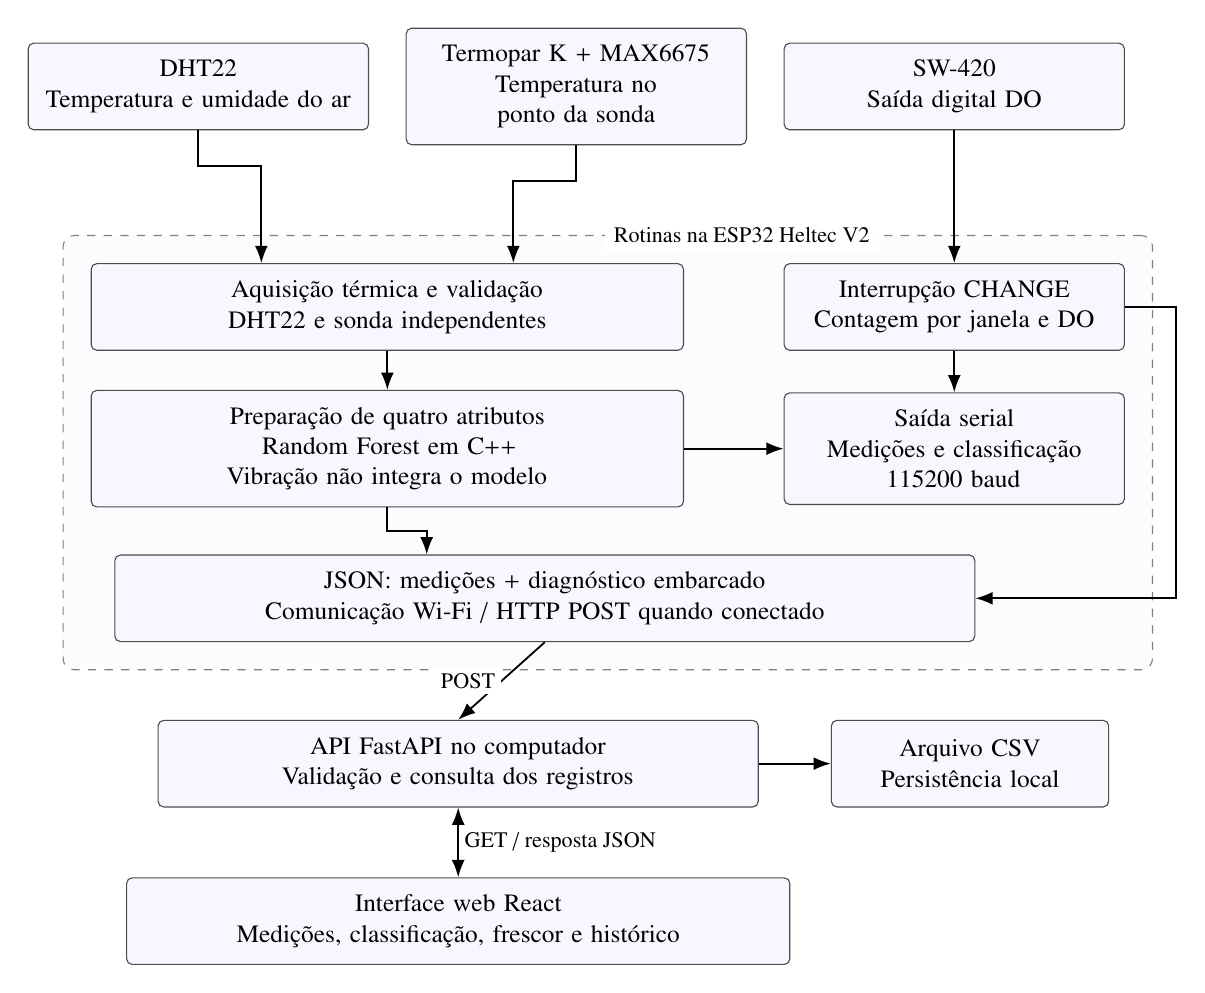
\begin{tikzpicture}[x=1cm,y=1cm]
\node[block,text width=3.9cm] (dht) at (-4.8,0.9) {DHT22\\Temperatura e umidade do ar};
\node[block,text width=3.9cm] (probe) at (0,0.9) {Termopar K + MAX6675\\Temperatura no ponto da sonda};
\node[block,text width=3.9cm] (sw) at (4.8,0.9) {SW-420\\Saída digital DO};
\node[block,text width=7.1cm] (thermal) at (-2.4,-1.9) {Aquisição térmica e validação\\DHT22 e sonda independentes};
\node[block,text width=3.9cm] (count) at (4.8,-1.9) {Interrupção CHANGE\\Contagem por janela e DO};
\node[block,text width=7.1cm] (ai) at (-2.4,-3.7) {Preparação de quatro atributos\\Random Forest em C++\\Vibração não integra o modelo};
\node[block,text width=3.9cm] (serial) at (4.8,-3.7) {Saída serial\\Medições e classificação\\115200 baud};
\node[block,text width=10.5cm] (packet) at (-0.4,-5.6) {JSON: medições + diagnóstico embarcado\\Comunicação Wi-Fi / HTTP POST quando conectado};
\begin{scope}[on background layer]
\node[draw=black!50,dashed,rounded corners,fill=blue!1,inner sep=0.35cm,
fit=(thermal)(count)(ai)(serial)(packet)] (esp) {};
\end{scope}
\node[font=\footnotesize,fill=white] at ($(esp.north)+(1.7,0)$) {Rotinas na ESP32 Heltec V2};
\node[block,text width=7.2cm] (api) at (-1.5,-7.7) {API FastAPI no computador\\Validação e consulta dos registros};
\node[block,text width=3.1cm] (csv) at (5.0,-7.7) {Arquivo CSV\\Persistência local};
\node[block,text width=8cm] (web) at (-1.5,-9.7) {Interface web React\\Medições, classificação, frescor e histórico};
\draw[flow] (dht.south) -- ++(0,-0.45) -| ([xshift=-1.6cm]thermal.north);
\draw[flow] (probe.south) -- ++(0,-0.45) -| ([xshift=1.6cm]thermal.north);
\draw[flow] (sw) -- (count);
\draw[flow] (thermal) -- (ai);
\draw[flow] (ai.east) -- (serial.west);
\draw[flow] (count) -- (serial);
\draw[flow] (ai.south) -- ++(0,-0.3) -| ([xshift=-1.5cm]packet.north);
\draw[flow] (count.east) -- ++(0.65,0) |- (packet.east);
\draw[flow] (packet.south) -- (api.north) node[midway,left,edge label] {POST};
\draw[flow] (api) -- (csv);
\draw[{Latex[length=2.2mm]}-{Latex[length=2.2mm]},line width=0.65pt]
  (api.south) -- (web.north) node[midway,right,edge label] {GET / resposta JSON};
\end{tikzpicture}
}
\source{elaboração própria a partir do firmware, da API e do frontend do MS-Monitor}
\end{figure}

\begin{table}[htbp]
\centering
\caption{Responsabilidade dos módulos e limites da implementação}
\label{tab:modulos}
\small
\begin{tabularx}{\textwidth}{L{3cm}Y}
\toprule
Módulo & Função no protótipo\\
\midrule
Aquisição & Ler DHT22 e MAX6675; capturar mudanças do sinal digital de vibração por interrupção.\\
Pré-processamento & Validar as entradas, preservar indicadores de falha e calcular a diferença entre temperaturas.\\
IA embarcada & Executar o Random Forest exportado; produzir classe, índice, confiança e duração da chamada.\\
Interface local & Registrar medições e resultado na serial a 115200 baud, inclusive sem Wi-Fi.\\
Comunicação & Realizar uma tentativa de POST por leitura quando houver Wi-Fi; tratar o código de retorno.\\
API e armazenamento & Validar o contrato, registrar cada POST aceito em CSV e disponibilizar consultas.\\
Visualização & Exibir medições, origem da classificação, frescor dos dados e histórico no navegador.\\
Atuação & Não implementada; não há comando de ventilador no firmware atual.\\
\bottomrule
\end{tabularx}
\source{elaboração própria a partir do código do projeto}
\end{table}

\subsection{Caminhos de energia e de retorno}

A alimentação adotada é USB, com entrada nominal de 5~V na placa e
distribuição de 3,3~V aos módulos sensores. O terra é comum, conforme
a Figura~\ref{fig:alimentacao}. As linhas de alimentação e GND não representam
o fluxo lógico de dados. O termopar é passivo e se conecta às entradas
próprias do MAX6675; não recebe alimentação de 3,3~V na ponta sensora.

\begin{figure}[htbp]
\centering
\caption{Distribuição de alimentação adotada e referência de terra comum}
\label{fig:alimentacao}
\resizebox{\textwidth}{!}{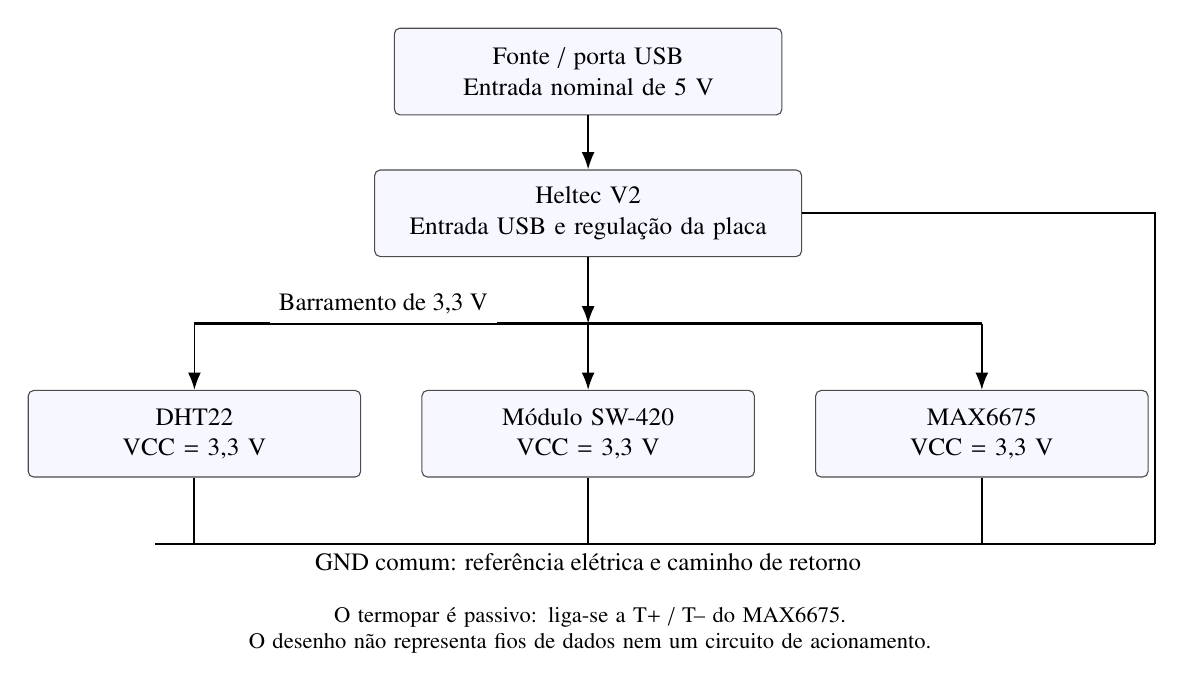
\begin{tikzpicture}[x=1cm,y=1cm]
\node[block,text width=4.5cm] (usb) at (0,0) {Fonte / porta USB\\Entrada nominal de 5 V};
\node[block,text width=5cm] (board) at (0,-1.8) {Heltec V2\\Entrada USB e regulação da placa};
\node[block,text width=3.8cm] (dht) at (-5,-4.6) {DHT22\\VCC = 3,3 V};
\node[block,text width=3.8cm] (sw) at (0,-4.6) {Módulo SW-420\\VCC = 3,3 V};
\node[block,text width=3.8cm] (max) at (5,-4.6) {MAX6675\\VCC = 3,3 V};
\draw[flow] (usb) -- (board);
\draw[line width=1pt] (-5,-3.2) -- (5,-3.2);
\draw[flow] (board.south) -- (0,-3.2);
\node[font=\small,fill=white,anchor=south] at (-2.6,-3.2) {Barramento de 3,3 V};
\foreach \target/\xx in {dht/-5,sw/0,max/5}{
  \draw[flow] (\xx,-3.2) -- (\target.north);
  \draw[line width=0.7pt] (\target.south) -- (\xx,-6);
}
\draw[line width=0.7pt] (-5.5,-6) -- (7.2,-6);
\draw[line width=0.7pt] (board.east) -- (7.2,-1.8) -- (7.2,-6);
\node[font=\small,fill=white,anchor=north] at (0,-6) {GND comum: referência elétrica e caminho de retorno};
\node[font=\footnotesize,align=center,text width=13cm] at (0,-7.1)
{O termopar é passivo: liga-se a T+ / T-- do MAX6675.\\
O desenho não representa fios de dados nem um circuito de acionamento.};
\end{tikzpicture}
}
\source{elaboração própria a partir das ligações documentadas; diagrama funcional, não esquema completo da placa}
\end{figure}

Os sinais que chegam aos GPIOs devem ser compatíveis com a lógica de
3,3~V da ESP32. A placa utilizada possui recursos adicionais de comunicação
e visualização, mas LoRa, Bluetooth e OLED não são utilizados pelo firmware
analisado \cite{heltecV2,espressif2026}. O GPIO~21, associado ao controle
de Vext nessa montagem, não é destinado aos sensores.

\begin{table}[htbp]
\centering
\caption{Mapa de conexões utilizado no firmware}
\label{tab:pinos}
\begin{tabularx}{\textwidth}{L{4.0cm}L{2.3cm}Y}
\toprule
Sinal & GPIO & Interface e direção em relação à ESP32\\
\midrule
DHT22 --- DAT & 17 & Protocolo digital temporizado, bidirecional.\\
SW-420 --- DO & 22 & Entrada digital; interrupção em \texttt{CHANGE}.\\
MAX6675 --- SCK & 13 & Saída de relógio gerada por software.\\
MAX6675 --- CS & 23 & Saída de seleção do conversor.\\
MAX6675 --- SO & 39 & Entrada de dados; GPIO de entrada.\\
VCC dos módulos & --- & Barramento de 3,3~V.\\
GND dos módulos & --- & Retorno comum ao GND da placa.\\
\bottomrule
\end{tabularx}
\source{elaboração própria a partir das constantes e rotinas do firmware}
\end{table}

\subsection{Grandezas elétricas e dimensionamento pendente}

O dimensionamento final requer a identificação da fonte USB, a corrente
dos módulos efetivamente montados e os picos durante a comunicação. Esses
valores não foram determinados pelos testes de software. Assim, não se
apresenta uma soma de correntes hipotéticas como consumo medido do protótipo.
A potência de entrada deve ser obtida no mesmo ponto de medição:
\begin{equation}
P_{\mathrm{USB}} = V_{\mathrm{USB}} I_{\mathrm{USB}}.
\end{equation}
Já a potência entregue apenas aos sensores no barramento de 3,3~V é
\begin{equation}
P_{\mathrm{sensores}} =
3{,}3\left(I_{\mathrm{DHT22}}+I_{\mathrm{MAX6675}}+I_{\mathrm{SW420}}\right),
\end{equation}
com correntes em ampères e potência em watts. Essa expressão não inclui
todo o consumo da placa, nem as perdas de regulação.

Como exemplo exclusivamente didático, para um resistor ideal de
$10~\mathrm{k}\Omega$ submetido a 3,3~V, a Lei de Ohm fornece
\begin{equation}
I=\frac{V}{R}=\frac{3{,}3}{10\,000}
=0{,}00033~\mathrm{A}=0{,}33~\mathrm{mA}.
\end{equation}
Esse resistor não é apresentado como componente identificado da montagem.
O exemplo apenas ilustra a relação entre tensão, resistência e corrente.
O plano de testes da Seção~\ref{sec:avaliacao} prevê a medição da entrada
USB e do barramento de 3,3~V antes de concluir sobre a suficiência da fonte.
\FloatBarrier

\section{Aquisição e preparação dos sinais}
\label{sec:aquisicao}

\subsection{Características dos componentes}

A Tabela~\ref{tab:componentes} reúne informações de referência e decisões da
montagem. Especificações de catálogo não equivalem a erros determinados no
protótipo: posicionamento, fiação, alimentação e características do módulo
podem afetar as leituras. Também é necessário distinguir resolução digital,
erro especificado e incerteza de uma comparação experimental.

\begin{table}[htbp]
\centering
\caption{Características técnicas relevantes ao protótipo}
\label{tab:componentes}
\small
\begin{tabularx}{\textwidth}{L{2.7cm}Y Y}
\toprule
Componente & Características de referência & Uso e limitação no projeto\\
\midrule
Heltec WiFi LoRa 32 V2 &
ESP32 clássico, dois núcleos LX6 até 240~MHz, 520~KiB de SRAM no chip e
8~MB de flash na placa; Wi-Fi de 2,4~GHz. &
Aquisição e inferência local. A memória disponível à aplicação depende
da partição e dos recursos do firmware.\\
DHT22 / AM2302 &
Temperatura de $-40$ a $80$\celsius; UR de 0 a 100\%; alimentação de
referência de 3 a 5~V; novas leituras em intervalos de pelo menos 2~s. &
Alimentado em 3,3~V. A referência consultada informa erro de
$\pm0{,}5$\celsius\ e de 2 a 5 pontos percentuais de UR; não aferidos no protótipo.\\
Termopar tipo K &
Sensor termoelétrico passivo; a conversão depende do MAX6675 e da
compensação da junção fria. &
Mede o ponto em que a ponta está instalada. Não caracteriza, sozinho,
o campo térmico de toda a massa de grãos.\\
MAX6675 &
Conversor de 12 bits, resolução de 0,25\celsius, alimentação de 3,0 a 5,5~V
e conversão de até 220~ms. &
Alimentado em 3,3~V; leitura serial por software. O código aceita
0 a 1024\celsius; o maior código de 12 bits equivale a 1023,75\celsius.\\
Módulo SW-420 &
Saída digital de um módulo de detecção de vibração; o ajuste e a
polaridade dependem da implementação utilizada. &
Alimentado em 3,3~V. Registra DO e transições; não fornece aceleração,
intensidade ou frequência mecânica calibradas.\\
\bottomrule
\end{tabularx}
\source{especificações de referência de Heltec, Espressif, Adafruit e Analog Devices; limites de uso extraídos do firmware \cite{heltecV2,espressif2026,adafruitDHT,max6675}}
\end{table}

No MAX6675, a resolução de 0,25\celsius\ não significa que o conjunto
termopar--conversor tenha esse erro máximo. O documento do fabricante
estabelece, por exemplo, erro do conversor de até 8~LSB na faixa de 0 a
700\celsius, com alimentação de 3,3~V e temperatura ambiente especificada,
além de tratar separadamente a compensação da junção fria
\cite{max6675}. Essas condições não constituem calibração da sonda montada.
Para o SW-420 não foi identificado um certificado ou uma especificação
metrológica do módulo efetivamente utilizado; por isso, não se atribuem
unidades físicas à contagem digital.

\subsection{Periodicidade e janela de vibração}

O firmware estabelece um intervalo nominal de 2500~ms. Na ausência de
atrasos adicionais, a taxa de ciclos é
\begin{equation}
f_{\mathrm{nominal}}=\frac{1}{2{,}5~\mathrm{s}}
=0{,}4~\mathrm{Hz},
\end{equation}
equivalente a aproximadamente 24 ciclos por minuto. Essa é a taxa nominal
de aquisição e envio, não uma frequência de amostragem de uma forma de
onda de vibração. A duração real é transmitida em \texttt{window\_ms},
pois atrasos de rede ou de execução podem prolongar a janela.

As transições do SW-420 são capturadas por uma interrupção em
\texttt{CHANGE}; o contador é copiado e reiniciado em seção crítica.
O fechamento da janela antecede a leitura dos sensores térmicos, portanto
o registro não deve ser descrito como uma aquisição simultânea de todas
as grandezas. A rotina de interrupção não faz HTTP, leitura do DHT22 ou
impressão serial. Como a biblioteca do DHT pode bloquear interrupções
brevemente, a contagem continua sendo uma medida demonstrativa.

A janela inicial também fornece tempo superior aos 220~ms de conversão
do MAX6675. A leitura ocorre uma vez por ciclo, utilizando o construtor
na ordem SCK, CS e SO. Não se pressupõe o uso de I$^{2}$C: o DHT22 usa
seu protocolo temporizado, e o MAX6675 utiliza uma interface serial
compatível com SPI implementada por software.

\subsection{Validação, atributos e tratamento de falhas}

O DHT22 é considerado válido quando temperatura e UR são finitas e estão
nos limites aceitos pelo firmware. Se falhar, ambos os valores são enviados
como \texttt{null}, com \texttt{dht\_ok=false}. A sonda é validada de forma
independente; termopar aberto pode resultar em \texttt{NAN} na biblioteca,
tratado como temperatura \texttt{null} e \texttt{probe\_ok=false}.
Temperatura igual a zero é uma entrada possível e não identifica falha.

Somente com os dois sensores térmicos válidos é preparado o vetor
\begin{equation}
\mathbf{x}=
\left[T_{\mathrm{ar}},\ \mathrm{UR}_{\mathrm{ar}},\
T_{\mathrm{sonda}},\ \Delta T\right],
\qquad
\Delta T=T_{\mathrm{sonda}}-T_{\mathrm{ar}}.
\label{eq:atributos}
\end{equation}
O pré-processamento reproduz operações em \texttt{float32}. A versão
embarcada não calcula médias móveis, espectro, tendências ou dias de
armazenamento como entradas da IA. Também não implementa filtragem
digital de vibração. Essas operações não devem ser atribuídas ao
protótipo apenas por aparecerem em propostas de evolução.

Uma falha térmica torna a classificação indisponível, sem reaproveitar
uma classe anterior como se fosse atual. A telemetria de vibração
continua sendo enviada. De modo recíproco, uma leitura de vibração
igual a zero não impede a inferência térmica.
\FloatBarrier

\section{Modelo de IA e implantação no firmware}
\label{sec:modelo}

\subsection{Treinamento no computador e inferência no dispositivo}

Random Forest combina diferentes árvores treinadas com aleatorização
de amostras e atributos \cite{breiman2001}. No projeto, o treinamento
foi implementado com scikit-learn \cite{pedregosa2011}. A configuração
compacta tem 32 árvores, profundidade máxima 6, mínimo de cinco amostras
por folha, balanceamento \texttt{balanced\_subsample} e semente 42.
Esses parâmetros e o relatório por classe constam do artefato técnico
\path{docs/embedded-ai-metrics.json}.

A Figura~\ref{fig:treinamento} diferencia treinamento, avaliação e
exportação. O script \path{ai/train_embedded.py} gera o cabeçalho
\path{firmware/ms_monitor/risk_model.h}. Os parâmetros aprendidos são
representados por tabelas constantes de nós e raízes; não são limiares
manuais definidos para inferir presença de fungos.
O arquivo \texttt{.joblib} é mantido no computador para reprodução e
comparação e não é carregado pela ESP32 nem pela API atual.

\begin{figure}[htbp]
\centering
\caption{Preparação do modelo embarcado e verificação da exportação}
\label{fig:treinamento}
\resizebox{0.96\textwidth}{!}{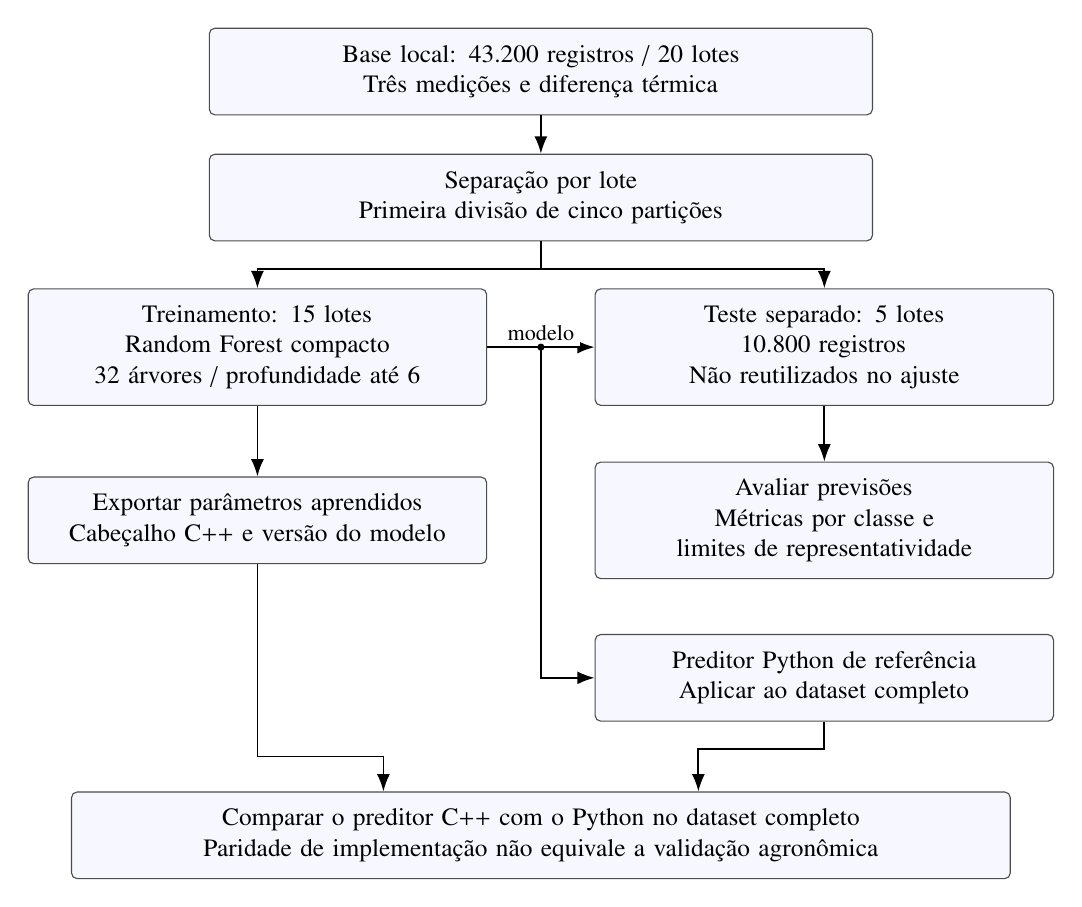
\begin{tikzpicture}[x=1cm,y=1cm]
\node[block,text width=8cm] (data) at (0,0)
{Base local: 43.200 registros / 20 lotes\\Três medições e diferença térmica};
\node[block,text width=8cm] (split) at (0,-1.6)
{Separação por lote\\Primeira divisão de cinco partições};
\node[block,text width=5.4cm] (train) at (-3.6,-3.5)
{Treinamento: 15 lotes\\Random Forest compacto\\32 árvores / profundidade até 6};
\node[block,text width=5.4cm] (test) at (3.6,-3.5)
{Teste separado: 5 lotes\\10.800 registros\\Não reutilizados no ajuste};
\node[block,text width=5.4cm] (export) at (-3.6,-5.7)
{Exportar parâmetros aprendidos\\Cabeçalho C++ e versão do modelo};
\node[block,text width=5.4cm] (metrics) at (3.6,-5.7)
{Avaliar previsões\\Métricas por classe e\\limites de representatividade};
\node[block,text width=5.4cm] (reference) at (3.6,-7.7)
{Preditor Python de referência\\Aplicar ao dataset completo};
\node[block,text width=11.5cm] (parity) at (0,-9.7)
{Comparar o preditor C++ com o Python no dataset completo\\
Paridade de implementação não equivale a validação agronômica};
\draw[flow] (data) -- (split);
\draw[flow] (split.south) -- ++(0,-0.35) -| (train.north);
\draw[flow] (split.south) -- ++(0,-0.35) -| (test.north);
\draw[flow] (train) -- (export);
\draw[flow] (test) -- (metrics);
\draw[flow] (train.east) -- (test.west) node[midway,above,edge label] {modelo};
\fill (0,-3.5) circle (1.3pt);
\draw[flow] (0,-3.5) -- (0,-7.7) -- (reference.west);
\draw[flow] (export.south) -- (-3.6,-8.7) -| ([xshift=-2cm]parity.north);
\draw[flow] (reference.south) -- ++(0,-0.35) -| ([xshift=2cm]parity.north);
\end{tikzpicture}
}
\source{elaboração própria a partir dos scripts de treinamento e verificação}
\end{figure}

Os dados locais são descritos na documentação como sintéticos: 43\,200
registros distribuídos em 20 lotes. Não há, no material examinado,
comprovação de que os rótulos derivem de análises microbiológicas
dos grãos do protótipo. A identificação do conjunto é preservada
por seu hash SHA-256 no relatório de treinamento.

O código usa a \textbf{primeira divisão} produzida por
\texttt{StratifiedGroupKFold} com cinco partições, mantendo lotes
inteiros separados. O experimento utiliza 32\,400 registros de 15
lotes no treinamento e 10\,800 registros de cinco lotes no teste.
Não se trata de uma média de desempenho de cinco rodadas de validação
cruzada, nem de uma validação temporal independente.

\subsection{Saídas do classificador e seu significado}

A execução retorna um dos rótulos \texttt{low}, \texttt{moderate},
\texttt{high} ou \texttt{critical}. Neste relatório, eles são
interpretados como níveis nominais do conjunto de treinamento,
respectivamente baixo, moderado, alto e crítico.
Esses nomes não estabelecem critérios agronômicos validados nem
recomendações automáticas de intervenção.

Para cada classe $c$, o preditor calcula a média das probabilidades
das folhas atingidas pelas $M=32$ árvores:
\begin{equation}
p_c(\mathbf{x})=\frac{1}{M}\sum_{m=1}^{M}p_{m,c}(\mathbf{x}),
\qquad
\widehat{c}=\arg\max_c p_c(\mathbf{x}).
\end{equation}
A confiança reportada é $\max_c p_c(\mathbf{x})$; não corresponde a
uma medida experimental de certeza sobre a condição sanitária do lote.
O índice apresentado em \texttt{risk\_score} segue a convenção
\begin{equation}
s=0\,p_{\mathrm{low}}+0{,}33\,p_{\mathrm{moderate}}
+0{,}66\,p_{\mathrm{high}}+1\,p_{\mathrm{critical}}.
\label{eq:score}
\end{equation}
Os pesos são uma escala de apresentação adotada no código. Mesmo
quando expresso como percentual no dashboard, $s$ não é uma
probabilidade calibrada de haver fungos ou micotoxinas.

\subsection{Execução e independência da rede}

O fluxo da Figura~\ref{fig:algoritmo} segue a ordem do firmware.
O tempo de inferência é medido ao redor da chamada local do preditor
com \texttt{micros()}, antes de verificar a conectividade.
Sem Wi-Fi, o dispositivo continua lendo os sensores, classificando
entradas válidas e registrando o resultado na serial. Os dados
desse período não são enfileirados para envio posterior.

Quando há rede, ocorre uma tentativa de POST por ciclo. O firmware
não testa antecipadamente a disponibilidade da API: interpreta a
resposta HTTP após tentar o envio. O código considera 201 como
aceitação e registra os demais códigos ou erros. Os limites
configurados são 700~ms para conexão e 1000~ms para leitura HTTP;
não representam garantia de latência total do ciclo.

\begin{figure}[p]
\centering
\caption{Fluxograma da aquisição e da inferência no firmware}
\label{fig:algoritmo}
\resizebox{0.94\textwidth}{!}{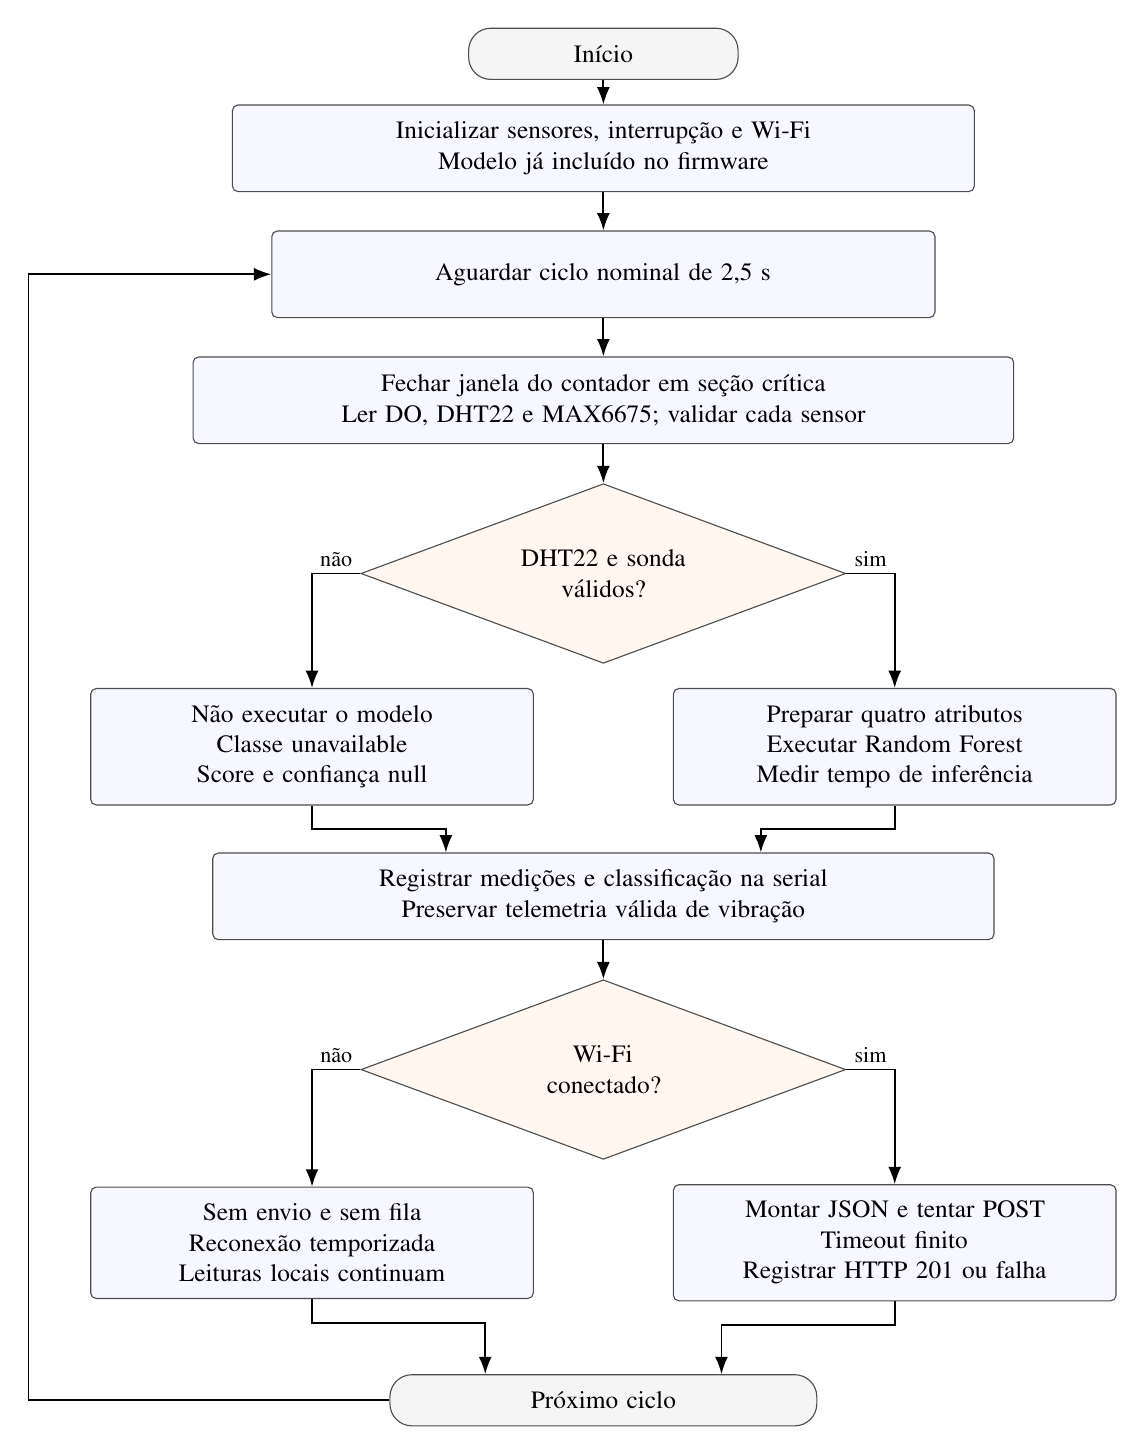
\begin{tikzpicture}[x=1cm,y=1cm]
\node[terminal,text width=3cm] (start) at (0,0) {Início};
\node[block,text width=9cm] (init) at (0,-1.2)
{Inicializar sensores, interrupção e Wi-Fi\\Modelo já incluído no firmware};
\node[block,text width=8cm] (wait) at (0,-2.8)
{Aguardar ciclo nominal de 2,5 s};
\node[block,text width=10cm] (read) at (0,-4.4)
{Fechar janela do contador em seção crítica\\Ler DO, DHT22 e MAX6675; validar cada sensor};
\node[decision,text width=4cm] (valid) at (0,-6.6)
{DHT22 e sonda\\válidos?};
\node[block,text width=5.2cm] (invalid) at (-3.7,-8.8)
{Não executar o modelo\\Classe unavailable\\Score e confiança null};
\node[block,text width=5.2cm] (infer) at (3.7,-8.8)
{Preparar quatro atributos\\Executar Random Forest\\Medir tempo de inferência};
\node[block,text width=9.5cm] (serial) at (0,-10.7)
{Registrar medições e classificação na serial\\Preservar telemetria válida de vibração};
\node[decision,text width=4cm] (wifi) at (0,-12.9)
{Wi-Fi\\conectado?};
\node[block,text width=5.2cm] (offline) at (-3.7,-15.1)
{Sem envio e sem fila\\Reconexão temporizada\\Leituras locais continuam};
\node[block,text width=5.2cm] (post) at (3.7,-15.1)
{Montar JSON e tentar POST\\Timeout finito\\Registrar HTTP 201 ou falha};
\node[terminal,text width=5cm] (next) at (0,-17.1) {Próximo ciclo};
\draw[flow] (start) -- (init);
\draw[flow] (init) -- (wait);
\draw[flow] (wait) -- (read);
\draw[flow] (read) -- (valid);
\draw[flow] (valid.west) -| (invalid.north) node[pos=0.25,above,edge label] {não};
\draw[flow] (valid.east) -| (infer.north) node[pos=0.25,above,edge label] {sim};
\draw[flow] (invalid.south) -- ++(0,-0.3) -| ([xshift=-2cm]serial.north);
\draw[flow] (infer.south) -- ++(0,-0.3) -| ([xshift=2cm]serial.north);
\draw[flow] (serial) -- (wifi);
\draw[flow] (wifi.west) -| (offline.north) node[pos=0.25,above,edge label] {não};
\draw[flow] (wifi.east) -| (post.north) node[pos=0.25,above,edge label] {sim};
\draw[flow] (offline.south) -- ++(0,-0.3) -| ([xshift=-1.5cm]next.north);
\draw[flow] (post.south) -- ++(0,-0.3) -| ([xshift=1.5cm]next.north);
\draw[flow] (next.west) -- (-7.3,-17.1) -- (-7.3,-2.8) -- (wait.west);
\end{tikzpicture}
}
\source{elaboração própria a partir de \texttt{ms\_monitor.ino}; a rotina de interrupção do SW-420 opera em paralelo ao ciclo principal}
\end{figure}

O modelo embarcado é identificado como \modelversion. O relatório de
compilação registrado no projeto, para core Espressif 3.3.12 e
FQBN \path{esp32:esp32:heltec_wifi_lora_32_V2}, informa
1\,043\,428 bytes de programa, diante de um limite de 3\,342\,336 bytes,
e 48\,824 bytes de variáveis globais na região de 327\,680 bytes
contabilizada pela ferramenta. As tabelas de nós e raízes ocupam
102\,496 bytes no compilador nativo de verificação.

Esses números sustentam a análise de compatibilidade da compilação,
mas não medem o heap livre em execução, a duração da inferência
na placa ou o consumo elétrico. Tampouco se deve confundir a região
de memória descrita pelo compilador com a SRAM física total do chip.
\FloatBarrier

\section{Comunicação, armazenamento e visualização}
\label{sec:comunicacao}

\subsection{Contrato de transmissão}

O envio é realizado pela ESP32 em rede Wi-Fi de 2,4~GHz, por
\texttt{POST /api/readings}. A API valida tipos, limites e coerência
dos indicadores de falha; um registro aceito e persistido retorna HTTP~201.
Payloads incompatíveis retornam 422. Falha de gravação do CSV retorna
503, sem substituir a última leitura aceita.
O Código~\ref{cod:payload} utiliza os nomes efetivamente exigidos
pelo contrato atual.

\begin{lstlisting}[caption={Payload ilustrativo compatível com o contrato da API},label={cod:payload}]
{
  "device_id": "ms-monitor-g3",
  "uptime_ms": 125000,
  "window_ms": 2500,
  "temperature_c": 24.8,
  "humidity_pct": 59.2,
  "dht_ok": true,
  "probe_temperature_c": 25.25,
  "probe_ok": true,
  "vibration_do": 0,
  "vibration_transitions": 12,
  "embedded_diagnosis": {
    "source": "esp32",
    "model_version": "embedded-rf-6b0d1696547d",
    "risk_level": "low",
    "risk_score": 0.12,
    "confidence": 0.8,
    "inference_us": 123
  }
}
\end{lstlisting}

Todos os valores desse exemplo são \textbf{ilustrativos}. Em particular,
123~$\mu$s não é uma duração medida na placa. O objeto exemplifica o
contrato, e não um ensaio físico. A diferença térmica é calculada
internamente para a IA e não constitui um campo próprio no POST atual.

O campo \texttt{uptime\_ms} representa tempo desde a inicialização da placa,
não horário civil. O servidor acrescenta \texttt{received\_at} em UTC.
Esse carimbo corresponde ao recebimento, sujeito ao atraso de comunicação,
e não ao instante exato de aquisição. A API não executa outra inferência:
apenas valida e prepara o diagnóstico recebido para exibição.

\subsection{Consulta e persistência}

\begin{table}[htbp]
\centering
\caption{Interfaces HTTP implementadas}
\label{tab:api}
\small
\begin{tabularx}{\textwidth}{L{5.0cm}Y}
\toprule
Rota & Finalidade\\
\midrule
\texttt{GET /health} & Saúde da API, independente do estado do dispositivo.\\
\texttt{POST /api/readings} & Recebimento e persistência de uma leitura e de seu diagnóstico embarcado.\\
\texttt{GET /api/readings/latest} & Última leitura, idade, estado de atualização e diagnóstico recebido.\\
\texttt{GET /api/readings?limit=300} & Histórico, em ordem cronológica, com limite de 1 a 3600 registros.\\
\texttt{GET /api/readings/export} & Download do CSV completo até o instante da solicitação.\\
\bottomrule
\end{tabularx}
\source{elaboração própria a partir de \texttt{backend/app.py}}
\end{table}

O arquivo padrão é \path{backend/data/readings.csv}. Cada POST aceito
gera uma linha com as medições, os indicadores de validade e os campos
\path{ai_source}, \path{ai_model_version}, \path{ai_risk_level},
\path{ai_risk_score}, \path{ai_confidence} e
\path{ai_inference_us}. Campos ausentes ficam em branco no CSV.
As colunas de IA registram previsões, e não rótulos independentes de
contaminação para treinamento supervisionado.

O histórico em memória é limitado aos últimos 3600 registros e é
recuperado do CSV ao iniciar a API. O arquivo completo continua crescendo,
portanto a coleta exige acompanhamento do espaço em disco e cópias de
segurança. Deve haver uma única instância da API, com um único worker,
por arquivo. Após reiniciar, o histórico permanece disponível, mas o
estado da última leitura aguarda um novo envio.

O envelope de consulta diferencia \texttt{waiting}, antes de um POST
aceito pela instância, \texttt{online}, para leitura com idade inferior
a 10~s, e \texttt{stale}, a partir desse intervalo. O frescor é calculado
por tempo monotônico no servidor. Um dispositivo com dados recentes
ainda pode reportar falha de um sensor; por isso, conectividade e
validade das medições são informações distintas.

\subsection{Apresentação e limites de comunicação}

O dashboard exibe temperatura do ar, temperatura da sonda, UR,
transições por janela, última atualização e resultado embarcado com
versão e tempo de inferência. A diferença térmica é uma entrada
interna do modelo, não um card dedicado na interface examinada.
O card de ventilação permanece como \textit{Não avaliado}.

Para os valores ilustrativos do Código~\ref{cod:payload}, a interface
apresentaria 24,8\celsius\ de temperatura do ar, 59,2\% de UR,
25,25\celsius\ na sonda e 12 transições em uma janela de 2,5~s,
com DO igual a zero. A classe \texttt{low} apareceria como
\textit{Baixo risco}, com índice de 12\%, confiança de 80\% e
inferência de 123~$\mu$s. Essa correspondência exemplifica a
formatação dos dados recebidos, sem transformar o exemplo em
resultado de ensaio ou o índice em confirmação de contaminação.

A última leitura é consultada aproximadamente a cada segundo; o
histórico é sincronizado de forma independente. O modo \textit{Ao vivo}
prioriza a coleta atual, enquanto o histórico e o CSV preservam
registros anteriores. Uma pausa de recepção não é preenchida com
valores artificiais. Na indisponibilidade da API, os valores anteriores
continuam visíveis com indicação de desatualização.

A API local usa HTTP e não implementa autenticação de dispositivos.
CORS restringe origens de navegador, mas não autentica POSTs enviados
pela ESP32. A arquitetura não deve ser apresentada como solução de
segurança para acesso público à internet. Credenciais de Wi-Fi ficam
em um \texttt{config.h} local e não integram o repositório ou este relatório.
\FloatBarrier

\section{Evidências disponíveis e plano de testes}
\label{sec:avaliacao}

\subsection{Resultados computacionais do modelo}

As métricas da Tabela~\ref{tab:metricas} são provenientes da avaliação
registrada para o modelo compacto, nos lotes de teste descritos na
Seção~\ref{sec:modelo}. Elas avaliam correspondência com rótulos do
dataset local, não detecção experimental de fungos no mini-silo.

\begin{table}[htbp]
\centering
\caption{Avaliação do modelo no conjunto de teste}
\label{tab:metricas}
\begin{tabularx}{\textwidth}{Y L{5.8cm}}
\toprule
Indicador & Resultado\\
\midrule
Registros de teste & 10\,800\\
Acurácia geral do Random Forest & 98,9907\%\\
Acurácia balanceada & 49,9860\%\\
F1 macro, considerando quatro rótulos & 24,8732\%\\
Acurácia de prever sempre \texttt{low} & 99,0185\%\\
\bottomrule
\end{tabularx}
\source{relatório \texttt{embedded-ai-metrics.json}; referência constante calculada pela proporção da classe \texttt{low}}
\end{table}

\begin{table}[htbp]
\centering
\caption{Representatividade das classes no teste e sensibilidade observada}
\label{tab:classes}
\begin{tabularx}{\textwidth}{L{2.7cm}L{2.4cm}L{3cm}Y}
\toprule
Rótulo & Suporte & Recall & Interpretação\\
\midrule
\texttt{low} & 10\,694 & 99,9719\% & Classe amplamente predominante.\\
\texttt{moderate} & 106 & 0\% & Nenhum exemplo dessa classe foi reconhecido corretamente.\\
\texttt{high} & 0 & Não estimável & Ausente no conjunto de teste.\\
\texttt{critical} & 0 & Não estimável & Ausente no conjunto de teste.\\
\bottomrule
\end{tabularx}
\source{relatório de classificação do modelo compacto}
\end{table}

O conjunto é fortemente desbalanceado. Uma decisão constante pela
classe \texttt{low} alcançaria
$10\,694/10\,800\approx99{,}02\%$, ligeiramente acima da acurácia
do modelo. Portanto, a acurácia geral elevada não demonstra vantagem
preditiva nesse teste. O recall nulo de \texttt{moderate} impede
afirmar que o classificador reconhece adequadamente os níveis
intermediários.

Há também uma diferença de cálculo entre os indicadores. O F1 macro
reportado inclui os quatro rótulos, atribuindo zero a resultados
indefinidos pela convenção \texttt{zero\_division=0}. A acurácia
balanceada corresponde à média dos recalls das classes presentes
no teste. Não se devem interpretar esses percentuais como avaliação
representativa das quatro condições. Para \texttt{high} e
\texttt{critical}, suporte zero significa falta de evidência,
não demonstração de erro ou acerto nessas condições.

\subsection{Verificação de software e da exportação}

Na revisão do relatório, foram executados 87 testes de backend e IA,
sete testes do frontend e o build TypeScript/Vite. As verificações
abrangem validação do contrato, compatibilidade com firmware anterior,
falhas independentes dos sensores, origem do diagnóstico, persistência
CSV e atualização do histórico. A existência de testes aprovados
não constitui validação metrológica ou biológica.

O script de verificação compilou o preditor C++ em ambiente nativo
e o comparou com o modelo Python em 43\,200 registros. Não houve
divergência de classe, e a maior diferença de probabilidade foi de
aproximadamente $3{,}01\times10^{-8}$. Trata-se de evidência de
fidelidade da exportação. Essa comparação inclui dados de treinamento
e, por isso, não é outra estimativa de generalização do modelo.

O registro de compilação da Heltec V2 descrito na
Seção~\ref{sec:modelo} é uma evidência distinta da comparação nativa.
Não foram realizados, nesta revisão documental, gravação de firmware, ensaio de
calibração, medição de consumo ou cronometragem de inferência na placa.
Essas tarefas permanecem no plano experimental.

\subsection{Plano de testes físicos e de integração}

As Tabelas~\ref{tab:testes} e~\ref{tab:testes-integracao} definem procedimentos e critérios a serem
registrados, sem apresentá-los como resultados já alcançados.
Instrumentos de referência devem ter sua identificação e condição
de calibração documentadas. Antes dos ensaios, devem ser registrados
espécie e massa dos grãos, geometria do mini-silo, posição dos
sensores e condições ambientais; esses elementos não estão
caracterizados no material técnico examinado.

\begin{table}[htbp]
\centering\small
\caption{Plano de verificação dos componentes e das falhas}
\label{tab:testes}
\begin{tabularx}{\textwidth}{L{2.5cm}Y Y}
\toprule
Objeto & Procedimento e instrumento & Evidência a registrar\\
\midrule
Alimentação &
Medir entrada USB e barramento de 3,3~V com multímetro; observar quedas
durante transmissão com osciloscópio, se disponível. &
Tensão mínima/máxima, corrente média e picos observáveis; confrontar com
a fonte e o regulador efetivos. Não inferir picos apenas da média.\\
DHT22 &
Comparar temperatura e UR com termo-higrômetro de referência em condições
estáveis e após mudança controlada de ambiente. &
Diferenças entre instrumentos, dispersão, tempo de estabilização e
ocorrência de leituras inválidas. Não confundir concordância pontual com calibração.\\
Sonda e MAX6675 &
Observar repouso, aquecer levemente a ponta com a mão e aguardar
estabilização; comparar com termômetro de referência em pontos adequados
à montagem. Verificar termopar aberto. &
Resposta térmica, diferença em relação à referência e sinalização
\texttt{probe\_ok=false}. Um valor numérico isolado não comprova exatidão.\\
SW-420 &
Aplicar perturbações reproduzíveis na estrutura; observar DO e transições
com analisador lógico, quando disponível. &
Polaridade, limiar ajustado, janela real e repetibilidade. Não converter
contagem em intensidade, RPM ou estado de ventilação.\\
Falhas e IA &
Introduzir falhas independentes de DHT22 e termopar, preservando conexões
seguras; conferir o payload e a serial. &
Medições inválidas null, classe \texttt{unavailable}, score/confiança
null e continuidade da telemetria válida de vibração.\\
\bottomrule
\end{tabularx}
\source{elaboração própria; plano de trabalho, sem resultado físico presumido}
\end{table}

\begin{table}[htbp]
\centering\small
\caption{Plano de verificação da integração e da validade do classificador}
\label{tab:testes-integracao}
\begin{tabularx}{\textwidth}{L{2.5cm}Y Y}
\toprule
Objeto & Procedimento e instrumento & Evidência a registrar\\
\midrule
Execução local &
Com sensores válidos, observar serial e interromper o Wi-Fi;
registrar a duração da inferência e memória livre em execução. &
Classificação local sem depender da API; distribuição de tempos
de \texttt{inference\_us}, reinicializações e comportamento do heap.\\
Rede e API &
Interromper/restabelecer Wi-Fi e servidor; enviar payloads válidos
e inválidos em ambiente de teste isolado. &
Retornos 201/422/503 quando aplicáveis, estados de frescor,
reconexão e inexistência de classificação reapresentada como nova.\\
CSV e interface &
Reiniciar a API, consultar o histórico, exportar o CSV e interromper a
rede do navegador durante uma coleta de teste. &
Persistência das linhas aceitas, indicadores de validade, origem
\texttt{esp32}, preservação de dados antigos e atualização de novos pontos.\\
Validade do classificador &
Definir protocolo de coleta por lotes independentes, com referências
físicas e, quando cabível, análise microbiológica por laboratório habilitado. &
Rótulos externos às previsões, matriz de confusão, recall por classe,
incerteza das métricas e avaliação de lotes não usados no ajuste.\\
\bottomrule
\end{tabularx}
\source{elaboração própria; plano de trabalho, sem resultado físico presumido}
\end{table}

Para investigar fungos, os rótulos futuros não devem ser produzidos
apenas pela própria temperatura ou pela classe prevista pelo modelo:
isso criaria uma avaliação circular. A aquisição ambiental e a
determinação de referência devem ser independentes. O planejamento
também deve considerar variações de tipo de grão, teor de água,
localização da sonda e fontes externas de aquecimento.
\FloatBarrier

\section{Conclusões sobre a viabilidade da arquitetura}

A revisão do MS-Monitor identifica uma arquitetura coerente para
aquisição de medições, execução local de um classificador compacto,
comunicação por HTTP e persistência dos registros. O código separa
a telemetria de vibração dos atributos térmicos e higrométricos,
trata falhas dos sensores e permite inferência local independente
do envio pela rede. A compilação registrada e a comparação
Python--C++ sustentam a viabilidade computacional preliminar.

Essa conclusão é limitada à implementação e às verificações descritas.
Não demonstra desempenho de detecção de fungos, contaminação ou
micotoxinas. O desbalanceamento do teste, a falta de exemplos de
duas classes e o recall nulo da classe moderada impedem atribuir
validade agronômica ao classificador atual. Seu uso apropriado,
nesta etapa, é a demonstração de aquisição, inferência embarcada
e integração de dados em uma atividade acadêmica.

A continuidade do projeto exige caracterização física da montagem,
comparação metrológica dos sensores, medição do consumo e avaliação
do tempo de inferência na ESP32. A investigação da relação com
condições de deterioração dependerá de dados experimentais
representativos e referências independentes. Controle e classificação
de ventilação permanecem fora da implementação analisada.

\section*{Declaração de apoio de inteligência artificial}

Ferramentas de IA generativa foram utilizadas como apoio à revisão
textual e técnica, à organização do documento LaTeX e à elaboração
de diagramas. As afirmações foram confrontadas com o código e as
fontes indicadas, e exemplos simulados foram identificados como tais.
Esse apoio não substitui a revisão dos integrantes, a avaliação
docente ou os ensaios experimentais. A responsabilidade pela versão
submetida permanece com os autores.

\clearpage
\phantomsection
\bibliographystyle{abntex2-alf}
\bibliography{referencias-relatorio}
\end{document}
